% !TeX spellcheck = en_US
\newpage
%%%%%%%%%%%%%%%%%%%%%%%%%%%%%%%%%%%%%%%%%%%%%%%%%%%%%%%%%%%%%%%%%%%%%%%%%%%
\section{Collision Detection}\index{Collision}
%%%%%%%%%%%%%%%%%%%%%%%%%%%%%%%%%%%%%%%%%%%%%%%%%%%%%%%%%%%%%%%%%%%%%%%%%%%
\subsection{Introduction}
Collision detection is used very often in game programming: characters must not walk through obstacles, projectiles hit targets, balls bounce off walls, and so on. For this reason, Pygame provides a whole variety of collision detection methods:

\begin{itemize}
	\item \textbf{Rectangle overlap}\index{collision detection!rectangle}: When we looked at the \texttt{Sprite} class, we already saw that the attribute \texttt{rect} is required.	It contains the position and size of the surrounding rectangle.	If two sprites meet, it is checked whether their rectangles overlap.	This is a very \emph{cheap} detection method, because only a few comparisons are needed to decide whether two rectangles touch or overlap. This method does not consider the actual shape of the sprite, only its bounding rectangle. Here is an example implementation:
	\lstset{firstnumber=1}
\begin{lstlisting}
def rectangle_collision(rect1, rect2):
   return rect1.left < rect2.right and
          rect2.left < rect1.right and
          rect1.top < rect2.bottom and
          rect2.top < rect1.bottom
\end{lstlisting}

\begin{figure}[H]
\begin{center}
\tikzset{
    shape rechteck/.style= {
    draw,
    line width = 1pt,
    inner xsep = 0.0cm,
    inner ysep = 0.0cm,
   }
}
\begin{tikzpicture}
\tiny
\draw [->, name=xachse] (0cm, 6cm)  -- +(13cm, 0cm);
\draw [<-, name=yachse] (0cm, 0cm)  -- +(0cm, 6cm);

\pgfsetfillopacity{0.5}
\draw (4.0cm, 3.0cm) node[name=k1,shape=rectangle,shape rechteck, fill = yellow!30, minimum height = 4.0cm, minimum width = 3cm] {};
\draw (6.5cm, 2.0cm) node[name=k2,shape=rectangle,shape rechteck, fill = green!30, minimum height = 3.5cm, minimum width = 5cm] {};
\pgfsetfillopacity{1.0}

\draw[-, very thick, red, dotted]  let \p1 = (k1.north west) in (k1.north west) --  (\x1, 6.0cm);
\draw[-, very thick, red, dotted]  let \p1 = (k1.north west) in (k1.north west) --  (0cm, \y1);
\draw[-, very thick, blue, dotted] let \p1 = (k1.north east) in (k1.north east) --  (\x1, 6.0cm);
\draw[-, very thick, blue, dotted] let \p1 = (k1.south west) in (k1.south west) --  (0cm,\y1);

\draw[-, very thick, red, dotted]  let \p1 = (k2.north west) in (k2.north west) --  (\x1, 6.0cm);
\draw[-, very thick, red, dotted]  let \p1 = (k2.north west) in (k2.north west) --  (0cm, \y1);
\draw[-, very thick, blue, dotted] let \p1 = (k2.north east) in (k2.north east) --  (\x1, 6.0cm);
\draw[-, very thick, blue, dotted] let \p1 = (k2.south west) in (k2.south west) --  (0cm,\y1);

\path [name=x1, color=red] let \p1 = (k1.north west) in node  at (\x1,6.4cm) {$left_1$};
\path [name=x2, color=red] let \p1 = (k2.north west) in node  at (\x1,6.4cm) {$left_2$};
\path [name=x1, color=blue] let \p1 = (k1.north east) in node  at (\x1,6.4cm) {$right_1$};
\path [name=x2, color=blue] let \p1 = (k2.north east) in node  at (\x1,6.4cm) {$right_2$};
\path [name=y1, color=red] let \p1 = (k1.north west) in node  at (-0.5cm,\y1) {$top_1$};
\path [name=y2, color=red] let \p1 = (k2.north west) in node  at (-0.5cm,\y1) {$top_2$};
\path [name=y1, color=blue] let \p1 = (k1.south west) in node  at (-0.9cm,\y1) {$bottom_1$};
\path [name=y2, color=blue] let \p1 = (k2.south west) in node  at (-0.9cm,\y1) {$bottom_2$};
\end{tikzpicture}
\caption{Collision detection with rectangles}\label{picKollRect01}
\end{center}
\end{figure}


	\item \textbf{Circle overlap}\index{collision detection!circle}: For rather round sprites, it is recommended not to check rectangles, but to use an bounding circle for collision detection instead. This collision test is also quite fast, because only the distance between the centers has to be compared:  $\sqrt{(x_2-x_1)^2+(y_2-y_1)^2} < r_1+r_2$. For performance reason the check is usually computed as: $(x_2-x_1)^2+(y_2-y_1)^2 < (r_1+r_2)^2$

\begin{figure}[H]
\begin{center}
\tikzset{
    shape kreis/.style= {
    draw,
    fill = yellow!30,
    line width = 1pt,
    inner xsep = 0.0cm,
    inner ysep = 0.0cm,
   }
}
\begin{tikzpicture}
\draw [->, name=xachse] (0cm, 0cm)  -- +(13cm, 0cm);
\draw [->, name=yachse] (0cm, 0cm)  -- +(0cm, 6cm);

\draw (4.0cm, 3.5cm) node[name=k1,shape=circle,shape kreis,  minimum height = 4cm] {};
\draw (8.5cm, 2.5cm) node[name=k2,shape=circle,shape kreis,  minimum height = 3cm] {};

\draw[-, very thick, blue] 
 (k1.north west) --  node[above, blue, xshift=0cm] {$r_1$} (k1.center);
\draw[-, very thick, blue] 
 (k2.north east) --  node[above, blue, xshift=0cm] {$r_2$} (k2.center);

\draw[-, very thick, blue] 
 (k1.center) --  node[above, blue, sloped, xshift=0cm] {\footnotesize$\sqrt{(x_2-x_1)^2+(y_2-y_1)^2}$} (k2.center);

\draw[-, very thick, red, dotted] 
 (k1.center) --  +(0cm, -3.5cm);
\draw[-, very thick, red, dotted] 
 (k1.center) --  +(-4.0cm, 0cm);

\draw[-, very thick, red, dotted] 
 (k2.center) --  +(0cm, -2.5cm);
\draw[-, very thick, red, dotted] 
 (k2.center) --  +(-8.5cm, 0cm);

\path [name=x1, color=red] let \p1 = (k1) in node  at (\x1,-0.4cm) {$x_1$};
\path [name=x2, color=red] let \p1 = (k2) in node  at (\x1,-0.4cm) {$x_2$};
\path [name=y1, color=red] let \p1 = (k1) in node  at (-0.4cm,\y1) {$y_1$};
\path [name=y2, color=red] let \p1 = (k2) in node  at (-0.4cm,\y1) {$y_2$};
\end{tikzpicture}
\caption{Collision detection with circles}\label{picKollKreis01}
\end{center}
\end{figure}

	\item \textbf{Pixel overlap}\index{collision detection!pixel}: In pixel-perfect collision detection, every pixel of both sprites is checked to see whether they occupy the same position.  If \emph{yes}, the sprites overlap; if \emph{no}, they do not.  This is the most expensive collision test, but also the most accurate one.  

	To reduce the computational effort, the intersection rectangle of the two sprites is determined first.  As with rectangle collision detection, it is first checked whether the two rectangles overlap at all. If they do not, the test can stop immediately.  If they do, the intersection of the two rectangles is itself a rectangle (see \abbref[vref]{picKollMask01}).  

\begin{figure}[H]
	\begin{center}
		\begin{tikzpicture}[font=\small, x=0.55cm, y=0.55cm]
			
			\tikzset{
				px/.style={draw, very thin, minimum width=0.55cm, minimum height=0.55cm},
				one/.style={px, fill=white},
				zero/.style={px, fill=black!12},
				ma/.style={px, fill=blue!20},
				mb/.style={px, fill=red!20},
				mab/.style={px, fill=green!20},
				title/.style={align=center, font=\bfseries}
			}
			
			% ---------------------------
			% Helper macro: draw a 6x6 mask with a set of "1" pixels
			% (#1 shift x, #2 shift y, #3 node prefix, #4 list of x/y ones)
			% ---------------------------
			\newcommand{\drawmask}[6]{%
				\begin{scope}[shift={(#1,#2)}]
					% grid 6x6: coords x=0..5, y=0..5, drawn top-down
					\foreach \x in {0,...,#6} {
						\foreach \y in {0,...,#6} {
							\node[zero] (#3-\x-\y) at (\x,-\y) {};
						}
					}
					% set ones
					\foreach \x/\y in {#5} {
						\node[#4] at (\x,-\y) {};
					}
				\end{scope}
			}
			
			% ---------------------------
			% Two masks (A and B)
			% ---------------------------
			\node[title] at (2.5,1.4) {Mask A};
			\node[title] at (11.5,1.4) {Mask B};
			\node[title] at (20.5,1.4) {Mask A $\cap$ Mask B};
			
			% Mask A at (0,0)
			\drawmask{0}{0}{A}{one}{
				2/1,3/1,
				1/2,2/2,3/2,4/2,
				1/3,2/3,3/3,4/3,
				2/4,3/4
			}{5}
			
			% Mask B 
			\drawmask{9}{0}{B}{one}{
				0/0,
				0/1,1/1,
				0/2,1/2,2/2,
				0/3,1/3,2/3,3/3,
				0/4,1/4,2/4,3/4,4/4,
				0/5,1/5,2/5,3/5,4/5,5/5
			}{5}
			
			% Mask A intersect Mask B
			\drawmask{18}{0}{A}{ma}{
				2/1,3/1,
				1/2,2/2,3/2,4/2,
				1/3,2/3,3/3,4/3,
				2/4,3/4
			}{5}
			\drawmask{20}{-2}{B}{mb}{
				0/0,
				0/1,1/1,
				0/2,1/2,2/2,
				0/3,1/3,2/3,3/3,
				0/4,1/4,2/4,3/4,4/4,
				0/5,1/5,2/5,3/5,4/5,5/5
			}{5}	
			\drawmask{20}{-2}{B}{mab}{
				0/0,
				0/1,1/1,
				0/2,1/2
			}{2}
			\begin{scope}[shift={(18,0)}]
				\foreach \x/\y in {2/1,3/1,1/2,2/2,3/2,4/2,1/3,2/3,3/3,4/3,2/4,3/4} 
				{
					\node[ma] at (\x,-\y) {};
				}
			\end{scope}
			\begin{scope}[shift={(20,-2)}]
				\foreach \x/\y in {0/0,0/1,1/1,0/2,1/2,2/2,0/3,1/3,2/3,3/3,0/4,1/4,2/4,3/4,4/4,0/5,1/5,2/5,3/5,4/5,5/5} 
				{
					\node[mb] at (\x,-\y) {};
				}
			\end{scope}
			\begin{scope}[shift={(20,-2)}]
				\foreach \x/\y in {0/0,0/1,1/1,0/2,1/2} 
				{
					\node[mab] at (\x,-\y) {};
				}
				\draw[very thick] (-0.5,0.5) rectangle (3.5,-3.5);
				\node[anchor=west] at (0, -6.0) {\small \textcolor{blue!80}{A has 1 here}};
				\node[anchor=west] at (0, -7.0) {\small \textcolor{red!80}{B has 1 here}};
				\node[anchor=west] at (0, -8.0) {\small \textcolor{green!80!black}{collision pixels (A AND B)}};
			\end{scope}
			
		\end{tikzpicture}
		\caption{Collision detection using masks}\label{picKollMask01}
	\end{center}
\end{figure}

	If two pixels have the same position, they must lie inside this intersection rectangle. Therefore, the pixel test can be limited to this usually much smaller area (see \abbref[vref]{picKollMask02}).  

	Another problem with pixel-perfect collision detection is distinguishing background from foreground. How should the collision test know whether a blue pixel belongs to the object or to the background?  There are several approaches to this problem.  The simplest one is to create a black-and-white image for each sprite (a \gls{mask}\index{mask}\randnotiz{mask});  the white pixels are relevant, while the black pixels can be ignored.  The pixel collision test is then performed only on these masks.

\begin{figure}[H]
	\begin{center}
		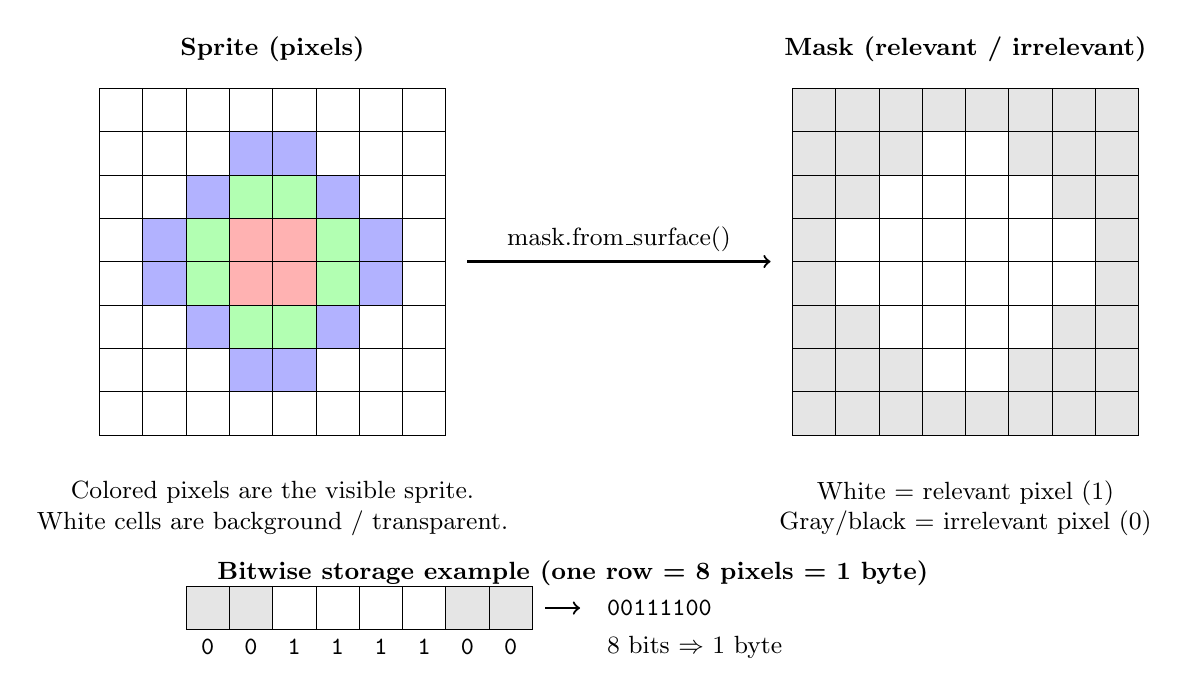
\begin{tikzpicture}[font=\small, x=0.55cm, y=0.55cm]
			
			% ---------- Parameters ----------
			\def\N{8} % grid size (NxN)
			
			% ---------- Titles ----------
			\node[align=center] (t1) at (3.5,1.4) {\textbf{Sprite (pixels)}};
			\node[align=center] (t2) at (19.5,1.4) {\textbf{Mask (relevant / irrelevant)}};
			
			% ---------- Helper styles ----------
			\tikzset{
				px/.style={draw, very thin, minimum width=0.55cm, minimum height=0.55cm},
				lbl/.style={align=center}
			}
			
			% ---------- SPRITE GRID (left) ----------
			% Draw an 8x8 pixel grid. We'll "paint" a circle-ish object.
			\begin{scope}[shift={(0,0)}]
				% Base grid
				\foreach \x in {0,...,7} {
					\foreach \y in {0,...,7} {
						\node[px, fill=white] (S-\x-\y) at (\x, -\y) {};
					}
				}
				
				% "Object" pixels (colored) - a simple round-ish blob
				\foreach \x/\y in {
					3/1,4/1,
					2/2,5/2,
					1/3,6/3,
					1/4,6/4,
					2/5,5/5,
					3/6,4/6
				}{
					\node[px, fill=blue!30] at (\x, -\y) {};
				}
				\foreach \x/\y in {
					3/2,4/2,
					2/3,5/3,
					2/4,5/4,
					3/5,4/5
				}{
					\node[px, fill=green!30] at (\x, -\y) {};
				}
				\foreach \x/\y in {
					3/3,4/3,
					3/4,4/4
				}{
					\node[px, fill=red!30] at (\x, -\y) {};
				}
				
				% Label note
				\node[lbl] at (3.5, -9.2) {Colored pixels are the visible sprite.\\White cells are background / transparent.};
			\end{scope}
			
			% ---------- MASK GRID (right) ----------
			\begin{scope}[shift={(16,0)}]
				% Base grid
				\foreach \x in {0,...,7} {
					\foreach \y in {0,...,7} {
						\node[px, fill=black!10] (M-\x-\y) at (\x, -\y) {};
					}
				}
				
				% Relevant pixels (white = 1)
				\foreach \x/\y in {
					3/1,4/1,
					2/2,3/2,4/2,5/2,
					1/3,2/3,3/3,4/3,5/3,6/3,
					1/4,2/4,3/4,4/4,5/4,6/4,
					2/5,3/5,4/5,5/5,
					3/6,4/6
				}{
					\node[px, fill=white] at (\x, -\y) {};
				}
				
				% Label note
				\node[lbl] at (3.5, -9.2) {White = relevant pixel (1)\\Gray/black = irrelevant pixel (0)};
			\end{scope}
			
			% ---------- Arrow between sprite and mask ----------
			\draw[->, thick] (8.0,-3.5) -- node[above]{mask.from\_surface()} (15.0,-3.5);
			
			% ---------- Bit encoding explanation (bottom) ----------
			% We show one row of 8 pixels and the corresponding 8 bits -> 1 byte.
			\begin{scope}[shift={(2,-11.5)}]
				\node[anchor=west] at (0,0.8) {\textbf{Bitwise storage example (one row = 8 pixels = 1 byte)}};
				
				% Draw 8 "mask pixels" for a row example
				\foreach \i/\bit in {0/0,1/0,2/1,3/1,4/1,5/1,6/0,7/0} {
					\node[px, fill={\ifnum\bit=1 white\else black!10\fi}] (R\i) at (\i,0) {};
					\node at (\i,-0.9) {\ttfamily\bit};
				}
				
				\node[anchor=west] at (9,0.0) {\ttfamily 00111100};
				
				\draw[->, thick] (7.8,0) -- (8.6,0);
				\node[anchor=west] at (9,-0.9) {8 bits $\Rightarrow$ 1 byte};
			\end{scope}
			
		\end{tikzpicture}
		\caption{From sprite to mask}\label{picKollMask02}
	\end{center}
\end{figure}


\end{itemize}


Let us look at the collision detection behaviour in more detail. In \abbref[vref]{piccollision00} we see four sprites: a wall, a spaceship, a monster, and a projectile. None of the sprites are touching each other.

In \abbref[vref]{piccollision01} you can clearly see the effect of collision detection using the bounding rectangles (bounding boxes). For the wall, everything is perfect: the projectile hits the wall, and the color indicates that the program has detected the collision.

However, we can also see the disadvantage when looking at the spaceship. A collision is detected even though the two sprites do not actually touch. The reason is that the spaceship’s bounding rectangle also includes the empty corners, so the rectangles overlap and a collision is reported. The same effect can also be observed with the monster.
 

\myezweihbild%
    {collision00.png}{0.38}{Four sprites\\\ }{piccollision00}%
    {collision01.png}{0.38}{Collision detection using rectangles (montage)}{piccollision01}


The situation is different when we use collision detection based on bounding circles (\abbref[vref]{piccollision02}). Now the collision with the wall is no longer detected correctly, because the corners of the wall do not belong to the inner circle. For the spaceship, however, this method produces exactly the desired result, since the empty corners are not part of the bounding circle. If we move a little further to the right, the spaceship would also turn red, because a collision would then be detected. The monster still produces an incorrect result.

Finally, there is pixel-perfect collision detection (\abbref[vref]{piccollision03}).  The collision with the wall is detected correctly. Even more interesting are the results for the spaceship and the monster. Both correctly report no collision, because the projectile is inside the rectangle and the inner circle, but only on transparent pixels. Feel free to try it yourself: move the projectile slightly to the left or right, and you will immediately see the pixel-perfect collision detection in action through the color change.

\myezweihbild%
    {collision02.png}{0.38}{Collision detection using circles (montage)}{piccollision02}%
    {collision03.png}{0.38}{Collision detection using masks (montage)}{piccollision03}


%%%%%%%%%%%%%%%%%%%%%%%%%%%%%%%%%%%%%%%%%%%%%%%%%%%%%%%%%%%%%%%%%%%%%%%%%%%
\subsection{More Input}
%%%%%%%%%%%%%%%%%%%%%%%%%%%%%%%%%%%%%%%%%%%%%%%%%%%%%%%%%%%%%%%%%%%%%%%%%%%
\subsubsection{Three Types of Collision Detection (of a Bullet)}
\begin{diskbox}
	\url{https://github.com/adamsralf/pygame_book/tree/main/src/00%20Introduction/08%20Collision/v01}
\end{diskbox}

Let us now take a closer look at the corresponding source code. However, I will skip another discussion of the \texttt{config.py}.

\lstsource{SRC/00 Introduction/08 Collision/v01/config.py}{1}{99}{python}{Collision types (1), \texttt{config.py}}{srcCollision00a} 

Things become more interesting with the \texttt{Obstacle} class. This class is used for the wall, the spaceship, and the monster.  For rectangle-based collision detection, the surrounding rectangle is required. As usual, it is obtained in \zeiref{srcCollision01} using \texttt{pygame.Surface.get\-\_rect()}\myindex{pyg}{\texttt{Surface}!\texttt{get\_rect()}}\randnotiz{get\_rect()} and stored in the attribute \texttt{rect}\index{self.rect}\randnotiz{self.rect}.  

For sprites with implicit transparency or explicit transparency set via \texttt{set\_colorkey()}\myindex{pyg}{\texttt{Surface}!\texttt{set\_colorkey()}}, the mask can be created very easily using \texttt{pygame.mask.from\_surface()}\myindex{pyg}{\texttt{mask}!\texttt{from\_surface()}}\randnotiz{from\_surface()} (\zeiref{srcCollision02}). In order for the predefined collision detection functions to work, this mask must be stored in the \texttt{Sprite} object using the attribute \texttt{mask}\index{self.mask}\randnotiz{self.mask}.  

In \zeiref{srcCollision03}, the bounding radius is calculated. This is implemented in a somewhat unclean way. Strictly speaking, one should determine the minimum of width and height and divide it by two. 

\lstset{firstnumber=15}
\begin{lstlisting}
self.radius = min(self.rect.width, self.rect.height) // 2
\end{lstlisting}

As with the mask, the radius must also be stored in an attribute so that the predefined collision methods can work: \texttt{radius}\index{self.radius|underline}\randnotiz{self.radius}.  

The flag \texttt{hit} is only used to ensure that the correct image is displayed depending on the detected collision. As you have probably already noticed, two images are loaded for these sprites: one for the \emph{not hit} state and one for the \emph{hit} state.

\lstsource{SRC/00 Introduction/08 Collision/v01/collision.py}{8}{24}{python}{Collision types (2), \texttt{Obstacle}}{srcCollision00b} 

The \texttt{Bullet} class is similar in many ways to the \texttt{Obstacle} class. Since we also want to use this class for all three types of collision detection, we need the same three attributes here as well: \texttt{rect}, \texttt{radius}, and \texttt{mask}.  

In addition, the class contains a few lines of code to allow the bullet to move; this should be self-explanatory. Note: for the sake of simplicity, no boundary check has been implemented. There is no real need for it here.


\lstsource{SRC/00 Introduction/08 Collision/v01/collision.py}{27}{48}{python}{Collision types (3), \texttt{Bullet}}{srcCollision00c} 

And now the \texttt{Game} class. In the constructor, the usual things happen. There is nothing particularly noteworthy here.

\lstsource{SRC/00 Introduction/08 Collision/v01/collision.py}{51}{65}{python}{Collision types (4), Constructor of \texttt{Game}}{srcCollision00d} 

The methods \texttt{run()} and \texttt{watch\_for\_events()} also follow well-established patterns.

\lstsource{SRC/00 Introduction/08 Collision/v01/collision.py}{67}{99}{python}{Collision types (5), \texttt{run()} and \texttt{watch\_for\_events()} of \texttt{Game}}{srcCollision00e} 

The same applies to the methods \texttt{update()} and \texttt{draw()}.

\lstsource{SRC/00 Introduction/08 Collision/v01/collision.py}{101}{112}{python}{Collision types (6), \texttt{update()} and \texttt{draw()} of \texttt{Game}}{srcCollision00f} 

The method \texttt{resize()} is not related to collision detection itself. Its only purpose is to ensure that the \texttt{Obstacle} objects are distributed evenly across the width of the window.  

The first \forSchleife\ calculates the total width of all \texttt{Obstacle} objects. This information is needed to compute the spacing in \zeiref{srcCollision04}. To do this, the total obstacle width is subtracted from the window width. The remaining number of pixels can then be distributed across the gaps.  

And how many gaps do we have? There are two gaps between the three \texttt{Obstacle} objects, one gap to the left border, and one to the right border -- a total of four gaps. The resulting spacing is stored in \texttt{padding}.  

In the second \forSchleife, the left position of each \texttt{Obstacle} object can then be calculated and set accordingly.


\lstsource{SRC/00 Introduction/08 Collision/v01/collision.py}{114}{123}{python}{Collision types (7), \texttt{resize()} of \texttt{Game}}{srcCollision00g} 

\begin{hintbox} [Drum roll]
And now the actual collision detection. Depending on which collision method we have selected, the corresponding collision function is called inside the \forSchleife: \texttt{pygame.sprite.col\-lide\-\_circle()}\myindex{pyg}{\texttt{sprite}!\texttt{collide\_circle()}|underline},  
\texttt{pygame.sprite.col\-lide\-\_mask()}\myindex{pyg}{\texttt{sprite}!\texttt{collide\_mask()}}, or  
\texttt{pygame.sprite.col\-lide\-\_rect()}\myindex{pyg}{\texttt{sprite}!\texttt{collide\_rect()}}.  
\end{hintbox}
 
The semantics are actually quite simple. Each of these methods is given two \texttt{Sprite} objects and returns \true\ if a collision is detected; otherwise it returns \false. As already mentioned above, it is important to ensure that the method being used can find the information it requires in the sprite:

\begin{hintbox}[Required information]
	\begin{itemize}
	    \item \texttt{pygame.sprite.collide\_circle()} needs \texttt{self.radius}
	    \item \texttt{pygame.sprite.collide\_mask()} needs \texttt{self.mask}
	    \item \texttt{pygame.sprite.collide\_rect()} needs \texttt{self.rect}
	\end{itemize}
\end{hintbox}

\newpage
\lstsource{SRC/00 Introduction/08 Collision/v01/collision.py}{125}{134}{python}{Collision types (8), \texttt{check\_for\_collision()} of \texttt{Game}}{srcCollision00h} 

%%%%%%%%%%%%%%%%%%%%%%%%%%%%%%%%%%%%%%%%%%%%%%%%%%%%%%%%%%%%%%%%%%%%%%%%%%%
\subsubsection{Checking all Sprites in a List}
\begin{diskbox}
	\url{https://github.com/adamsralf/pygame_book/tree/main/src/00%20Introduction/08%20Collision/v03}
\end{diskbox}

Rectangle-based collision detection between a single sprite and a list of sprites -- that is, checking whether one sprite collides with any sprite in a \texttt{SpriteGroup} -- is used so often that a dedicated method exists for this purpose: \texttt{pygame.sprite.spritecollide()}\myindex{pyg}{\texttt{sprite}!\texttt{spritecollide()}}\randnotiz{spritecollide()}.  

The first parameter is a single \texttt{Sprite} object -- in this case, our fireball. The second parameter is the list of sprites in which a collision should be checked. The third parameter controls whether the colliding objects should be removed from the list. This is very useful, for example, when an obstacle should disappear upon contact.

Below a minimal example (printed only partially). In \zeiref{srcCollision05a} the key part happens: one sprite -- \texttt{player} -- is checked for collisions with many sprites -- \texttt{blocks}. Every sprite that the player collides with is removed from all groups using \texttt{kill()}, and is therefore most likely deleted completely.

\lstsource{SRC/00 Introduction/08 Collision/v03/collision.py}{31}{62}{python}{\texttt{spritecollide()}}{srcCollision00i} 


%%%%%%%%%%%%%%%%%%%%%%%%%%%%%%%%%%%%%%%%%%%%%%%%%%%%%%%%%%%%%%%%%%%%%%%%%%%
\subsubsection{Using Function Pointer/Collision Callback}
\begin{diskbox}
	\url{https://github.com/adamsralf/pygame_book/tree/main/src/00%20Introduction/08%20Collision/v02}
\end{diskbox}

The method \texttt{pygame.sprite.spritecollide()} has a fourth parameter as well. This parameter can be used to pass a \gls{functionpointer}\index{function pointer}\randnotiz{function pointer} or \emph{collision callback}\index{collision callback}\randnotiz{collision callback} to a different collision detection method. This function must accept two \texttt{Sprite} objects as parameters.  

This means you can either use your own custom collision function or one of the three predefined methods: \texttt{collide\_circle()}, \texttt{collide\_mask()}, or \texttt{collide\_rect()}. If nothing is specified here -- as in our source code -- \texttt{collide\_rect()} is used automatically.

\lstsource{SRC/00 Introduction/08 Collision/v02/collision.py}{125}{135}{python}{Dynamic collision callback}{srcCollision01a} 


%%%%%%%%%%%%%%%%%%%%%%%%%%%%%%%%%%%%%%%%%%%%%%%%%%%%%%%%%%%%%%%%%%%%%%%%%%%
\newpage
\subsection{What was new?}

\begin{hintbox}
There are three standard ways to test the collision of two sprites: 
\begin{itemize}
	\item checking whether their rectangles intersect, 
	\item whether their bounding circles intersect, or 
	\item whether the pixels of the objects overlap.
\end{itemize}

In order to perform these collision tests, a sprite must provide the required information: \texttt{rect}, \texttt{radius}, or \texttt{mask}.
\end{hintbox}

\begin{figure}[H]
	\begin{center}
		\begin{tikzpicture}[>=Stealth, font=\small]
			
			% Axes
			\draw[->, thick] (0,0) -- (10,0) node[below right] {Cost};
			\draw[->, thick] (0,0) -- (0,7)  node[above left] {Accuracy};
			
			% Axis hints
			\node[below] at (2.0,0) {high};
			\node[below] at (8.0,0) {low};
			\node[left]  at (0,1.0) {low};
			\node[left]  at (0,6.5) {high};	
			
			% Rect (fast, inaccurate)
			\node[draw, rounded corners, align=left, fill=gray!10] (rect) at (7.8,1.3) {%
				\textbf{Rect}\\
				\texttt{collide\_rect}\\
				+ fastest\\
				-- sometimes improper 
			};
			
			% Circle (medium)
			\node[draw, rounded corners, align=left, fill=gray!10] (circle) at (5.3,3.6) {%
				\textbf{Circle}\\
				\texttt{collide\_circle}\\
				+ fast\\
				-- improper in corners
			};
			
			% Mask (accurate, expensive)
			\node[draw, rounded corners, align=left, fill=gray!10] (mask) at (2.5,5.8) {%
				\textbf{Mask}\\
				\texttt{collide\_mask}\\
				+ super precise\\
				-- most expensive
			};
		\end{tikzpicture}
		\caption[Tradeoff Accuracy vs. Costs]{\Gls{tradeoff} Accuracy vs. Costs}\label{picKollVergleich01}
	\end{center}
\end{figure}

\begin{pygbox}
\begin{itemize}
	\item \texttt{pygame.mask.from\_surface()}:
	\myindex{pyg}{\texttt{mask}!\texttt{from\_surface()}}\\ 
    \url{https://pyga.me/docs/ref/mask.html#pygame.mask.from_surface}
	
	\item \texttt{pygame.sprite.collide\_circle()}:
	\myindex{pyg}{\texttt{sprite}!\texttt{collide\_circle()}}\\ 
    \url{https://pyga.me/docs/ref/sprite.html#pygame.sprite.collide_circle}

	\item \texttt{pygame.sprite.collide\_mask()}:
	\myindex{pyg}{\texttt{sprite}!\texttt{collide\_mask()}}\\ 
    \url{https://pyga.me/docs/ref/sprite.html#pygame.sprite.collide_mask}

	\item \texttt{pygame.sprite.collide\_rect()}:
	\myindex{pyg}{\texttt{sprite}!\texttt{collide\_rect()}}\\ 
    \url{https://pyga.me/docs/ref/sprite.html#pygame.sprite.collide_rect}
	
	\item \texttt{pygame.sprite.spritecollide()}:
	\myindex{pyg}{\texttt{sprite}!\texttt{spritecollide()}}\\ 
    \url{https://pyga.me/docs/ref/sprite.html#pygame.sprite.spritecollide}
	
\end{itemize}
\end{pygbox}

%%%%%%%%%%%%%%%%%%%%%%%%%%%%%%%%%%%%%%%%%%%%%%%%%%%%%%%%%%%%%%%%%%%%%%%%%%%
\subsection{Homework}

\myebild{collision04.png}{0.5}{A simple collision game}{piccollision04}%

Create a game with the following properties:

\begin{enumerate}
	\item A player sprite is displayed at the bottom center of the playfield.
	
	\item The player can move in all four directions using the keyboard, but cannot leave the playfield.
	
	\item Thirty obstacles are placed on the playfield.
	
	\item Ten obstacles each are detected using rectangle collision, circle collision, and mask-based collision detection.
	
	\item The obstacles are placed in such a way that they do not overlap with each other or with the player.
	
	\item The obstacles move downward at different speeds.
	
	\item There is a score counter that starts at~0. It is to display on the top edge of the window.
	
	\item If an obstacle leaves the playfield at the bottom, it reappears at the top and the score counter is increased by~1.
	
	\item If an obstacle hits the player, the game is lost.
	
	\item Bonus: Over time, the obstacles become faster and faster.
	
	\item Bonus: A Game Over message and a restart option.
\end{enumerate}


